\section{為何會有香港人反對人大釋法?}
\label{sec:sec25}

因為程序很重要。人大釋法是指全國人民代表大會常務委員對《基本法》作出最終解釋。它之所以會在香港引發矛盾,甚至乎被視為對香港法治的挑戰,在於具體的實行方式和九七前香港社會的理解有明顯差別,運用範圍亦遠遠比想像中來得廣泛。由於人大釋法涉及香港高度自治的界線,所以市民會十分關注釋法的條件和香港法院在當中的角色,以符合三權分立的期望。人大釋法本來不一定有問題,但當它不按原來設想的程序發生,就引發了強烈反彈。

《基本法》第一百五十八條對釋法有這樣的定義:

\begin{displayquote}
    本法的解釋權屬於全國人民代表大會常務委員會。

    全國人民代表大會常務委員會授權香港特別行政區法院在審理案件時對本法關於香港特別行政區自治範圍內的條款自行解釋。

    香港特別行政區法院在審理案件時對本法的其他條款也可解釋。但如香港特別行政區法院在審理案件時需要對本法關於中央人民政府管理的事務或中央和香港特別行政區關係的條款進行解釋,而該條款的解釋又影響到案件的判決,在對該案件作出不可上訴的終局判決前,應由香港特別行政區終審法院請全國人民代表大會常務委員會對有關條款作出解釋。如全國人民代表大會常務委員會作出解釋,香港特別行政區法院在引用該條款時,應以全國人民代表大會常務委員會的解釋為準。但在此以前作出的判決不受影響。

    全國人民代表大會常務委員會在對本法進行解釋前,徵詢其所屬的香港特別行政區基本法委員會的意見。
\end{displayquote}

按字面的理解,釋法應按照以下程序:第一,如果法院認為事件屬香港自治範圍,就可以自己解釋。第二,如果法院認為事件屬中央人民政府管理的事務或中央和香港特別行政區關係,應由終審法院請全國人大常委解釋。第三,人大常委進行解釋前,應徵詢基本法委員會的意見。第四,解釋作出後香港法院須引用,但之前判決不受影響。

事實上,香港法院經常會自行解釋《基本法》的各項條文。例如終審法院在二零一三年就裁定了《婚姻訴訟條例》及《婚姻條例》不容許完成性別重整手術的女性與其男性伴侶註冊結婚,是違反了《基本法》第三十七條「香港居民的婚姻自由和自願生育的權利受法律保護」的規定,進而宣告《婚姻訴訟條例》中「女性」的涵義必須理解為包括已完成性別重整手術,並獲得醫學專家證明性別已經由男性改變為女性的人。

香港出現釋法爭議,是因為人大常委慣性繞過上述條文所描述的程序作出的釋法。事實上,在特區成立以來的五次人大釋法,就有四次不按上述程序發生。

這兒先由第一次釋法說起。一九九七年七月一日後的第一個星期,數以百計來自中國大陸的人士到入境處聲稱自己是香港永久性居民。事源《基本法》第二十四條規定,凡是香港永久性居民中的中國公民在香港以外所生的中國籍子女。於是乎,不少香港人在中國大陸所生的子女,包括不少非婚生子女,便在特區成立前以各種方式前來香港,並於特區成立後隨即向政府提出永久居民身分的申請。

香港政府當時擔心如果立即接納他們立即成為永久性居民,會引發一連串問題。例如婚生和非婚生子女有否分別,如何證明申請人真的是香港永久性居民的子女(特別是如果只有父親一方,而母親是他在中國大陸的情婦而非合法婦子),而以後類似的案例是否不用經單程證制度按配額排隊,而可直接前來香港。另一個極受爭議的問題,是這個資格是否可以即時世代相傳(例如某人出生時是中國大陸居民,他的父親也是,但他的祖父剛剛成為了香港永久性居民,則會否連帶其後代都會即時變成香港永久性居民)。

為了處理這些問題,臨時立法會在七月九日一天之內緊急立法,收緊了相關人士的入境安排,並追溯回到七月一日生效。此舉引來大量爭議,其中一名「無證兒童」吳嘉玲在父親代表下控告修訂違憲。到了一九九九年一月,終審法院就吳嘉玲作出裁決,表明香港永久性居民所生的子女不論婚生或非婚生,不論是否成年,不論有否單程證,亦不論是否生於內地,都可享有居港權。畢竟《基本法》的條文沒有就這些方面列明要求,也就不應限制。

對此裁決,政府推算可有於十年內有167萬人可從中國大陸移居香港,為香港社會帶來沉重壓力。儘管此推算被多方指為誇大,甚至是要製造恐慌影響公眾輿論,但政府仍以此為基礎謀求改變判決。到了一九九九年五月,政府決定正式提請人大常委就居港權釋法,而人大常委則於六月通過對《基本法》的第一次解釋。解釋內容列明即使是香港永久性居民在中國大陸所生的中國籍子女,進入香港前也要得到中國大陸方面的審批;而所謂香港永久性居民在香港以外所生的子女,是指出生時父或母已經符合香港永久性居民的規定。

這次釋法在香港司法界帶來極大震撼。首先,這次釋法不是由終審法院提出,而且是在終審法院已經作出最終判決之後才提出。如是者,終審法院從前不再「終審」,因為其最終判決原來是可以被中國政府推翻的,香港的自主性隨即被大幅削減。法律界當時就發起了黑衣靜默遊行抗議,後來更有解密文年指出終審法院五名常任法官曾經考慮集體辭職抗議。

及後的各次釋法,除了二零一一年因應外交事務而產生的第四次釋法,在香港都引起不少爭議。第二次釋法發生在二零零四年,人大常委在沒有終審法院或任何香港政治體制中的任何機關要求的情況下,主動就《基本法》附件一和附件二作出解釋,為香港未來的政治改革新增限制(見問題三十四)。此例一開,人大常委的釋法權在程序上已變成可隨時發生。第三次釋法發生在二零零五年,由首任行政長官董建華的辭職觸發,各界關注下一任行政長官的任期應為新一任行政長官,還是原有任期的續任。對此,署理行政長官曾蔭權在香港法院未有機會處理此爭議前,直接向人大常委尋求釋法,司法機構的角色再一次被矮化。

來到二零一六年的第五次釋法,其爭議程度更超越了之前四次的釋法。是次釋法的源起為有立法會議員於宣誓時涉嫌辱華,被立法會秘書長拒絕監誓而引發的政治風波(見問題二十二)。人大常委於一個月內旋即為《基本法》中有關公職人員宣誓的條文作出解釋,規範宣誓形式及內容,以及未進行合法有效宣誓、拒絕宣誓,或日後違反誓言的後果。從程序上來看,這此釋法最少有四個問題。第一,這次釋法並不是由終審法院提出,甚至連香港政府本身也不認為有需要釋法,原全是由人大常委自己提出。第二,這次釋法發生的時候,香港法庭正在處理政府和立法會就宣誓問題訴訟,政府代表要求禁止立法會主席為相開議員重新監誓。人大常委在此案的審議途中釋法,使得法庭連按原有程序考慮如何解釋《基本法》的機會也被剝奪,對香港司法程序極不尊重,也使條文中「之前判決不受影響」的規定變成形同虛設。第三,相關的《基本法》條文本身沒有提及宣誓的形式,但釋法的內容卻對此作詳細說明,形成了解釋《基本法》為名,增修《基本法》為實的客觀後果。如是者,《基本法》當中本來有關修改程序的規範條文亦變得形同虛設。而當《基本法》變得可以不按既定程序修改,整部《基本法》的權威地位也會因而消失。第四,《基本法》是憲法性文件,條文本應以本地立法的方式落實,例如宣誓形式的具體規範就是由《宣誓及聲明條例》列明。當人大釋法對宣誓形式的要求作出詳細說明,等於侵犯了立法會的本地立法職能。

在這次釋法當中,法治精神被矮化為僅僅是「當權力者以法律的形式來解決問題」,只要問題被解決了便行。因此,支持釋法的評論往往把其論證建基於「辱華是錯,所以釋法就是對」。不過,如果把法治的目的從「依法管治」提升到「以法限權」的層面,則莫論目的對錯,擁有權力者是否以適當的方式行使其權力,更為重要。這也是為什麼香港有不少輿論會認為香港法治因為歷次釋法而受到嚴重威脅,因他們正正是以「以法限權」來理解香港的法治(見\hyperref[sec:sec24]{問題二十四})。

\begin{figure}[htbp]
    \centering
    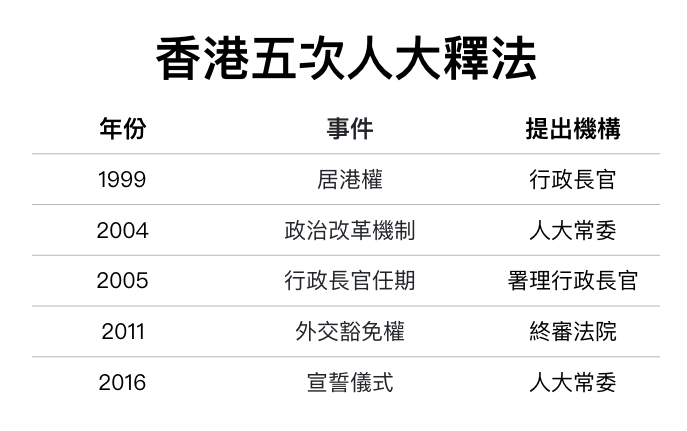
\includegraphics[width=0.7\textwidth]{c25/h-klesson1-041.png}
    \caption{五次釋法當中只有一次按《基本法》列明的程序發生}
\end{figure}

回看各次人大釋法的案例,今天香港社會對釋法的理解相對於九七前已大為不同。

首先,釋法程序不再一定要由香港的終審法院在有特定案件並認為此案件有需要的時候才能啟動,香港政府可以提出,人大常委也可以隨時自己提出。九七前對釋法程序的理解,是人大常委把釋法權授權與香港法院後,自己就不會再行駛此權力(這也是中國政府機關自己平時對授權的理解)。當這個理解被打破,第一百五十八條所描述的詳細程序就顯得多餘了。首次人大釋法時對此的解釋,是《基本法》第四十三條規定行政長官向中央人民政府負責的條文,把行政長官要求人大釋法理解為「就執行《基本法》有關條款所遇問題,向中央政府報告」。然而在此一理解下,香港的三權分立會受到嚴重打擊,因為日後行政權如若受到司法權的制衡,都可以上報國務院提請人大釋法。而司法權為免觸動人大釋法,監督行政權時便會變得有所顧忌,以免行政權駛出「絕招」。如是者,行政權和司法權之間便出現明顯的不平衡,權力逐漸會倒向行政權的一方。

第二,釋法的題目不再限於中央人民政府管理的事務或中央和香港特別行政區關係的條款,即使一些明顯屬於香港特別行政區自治範圍內的條款也可以隨時按人大常委的意願解釋。這樣會導致《基本法》對香港高度自治的保障一下子變得十分虛無,畢竟無論這些保障寫得如何細緻,也可以隨時被人大常委以解釋的名義推翻。如是者,每當香港出現重大爭議,無論是否和中港關係直接相關,大家就不再關心本地行政、立法和司法之間的相互制衡,而隨即問人大常委會不會以釋法作最後定論,本地的輿論和政治過程隨之被架空,也就脫離了「一國兩制、港人治港」的原意。

對於《基本法》中的釋法條文可以被中國政府任意引用,有意見認為這是《中英聯合聲明》的錯失。《中英聯合聲明》對香港很多基本政治制度都有所著墨,後來變成《基本法》的條文。但對於《基本法》的解釋權本身,《中英聯合聲明》卻沒有規範。有輿論認為草簽者當時沒有意識到《基本法》本身要面對中國法制和普通法制度之間的矛盾。

在普通法之下,香港法院獨立於政府運作,從法律文本去解釋條文(包括受爭議的條文和它與其他條文的關係),過程中不應作政治考慮,更不會增添文本本身沒有或不能包含的意思。在中國的法制下,中國《憲法》明文規定人大常委有權解釋所有法律,而人大常委作為一個政治而不是司法機構,則會考慮立法時的原意,考慮法律條文以外的資料,也可以因應法律制定後出現了的新情況為法律條文添加新的意思。

釋法之爭是程序之爭,但程序後面也是價值之爭。法治的價值,並不僅限於「合法就是法治」,畢竟美國的種族隔離政策曾己何時也是合法安排。法治所追求的,還有法律制訂的過程能否自我完善和達至公義。前文提及香港的行政權和立法權本身已有諸多制度缺陷,法庭作為制度內最後守門員的角色已經相當繁重和困難。當法庭的地位因釋法而被進一步削弱,社會對整個政治制度的信心就會進一步降低。

釋法之爭帶來一個十分令人擔憂的趨勢。社會中有不同意見和爭議,本來正常不過。如果香港有一個充分的民主制度,大可透過行政長官普選去決定社會要走的方向。當行政長官未能以民主選舉產生,市民便轉向靠立法會議員來表達不滿。當立法會也未能有效運作,市民便唯有通過司法覆核等方式請求司法機構主持正義。到了連司法機構也失去其應有地位,是否就代表社會不會再有爭議?當然不是。相反,當爭議無法在制度內得到有效處理,便會在制度外尋求出口,形成更難解決的社會矛盾。鯀禹治水,禹重堵截而禹重疏導,結果堵截帶來災難而疏導帶來盛世。特區的政治制度,至今卻是在每一個關口堵截民意,社會不穩自有其因。



伸延閱讀:

Chan JMM, Fu HL, Ghai Y, eds (2000) Hong Kong's Constitutional Debate: Conflict over Interpretation. Hong Kong: Hong Kong University Press.

Gittings D (2016) Interpretation and Amendment, \textit{Introduction to the Hong Kong Basic Law (2nd Edition)}. Hong Kong University Press.

Tai BYT (2012) Judiciary, \textit{Contemporary Hong Kong Government and Politics (Expanded Edition)}. Hong Kong University Press.